\chapter*{Estado del arte}
Para poder organizar este proyecto, debemos conocer el estado del arte en su ámbito. Como comentamos en la introducción, cheminformatics es un tema muy amplio y engloba subtópicos diferentes. Muchos de ellos surgieron en la década de 1960 y principios de 1970, y desde esa época muchos grupos de investigación siguen trabajando en ellos y nuevos grupos han surgido para aplicar nuevas tecnologías en nuevos ámbitos. A continuación discutimos algunos de los temas que históricamente han sido de interés para esta ciencia. \cite{doi:10.1021/ci600234z}

\section*{Representación de compuestos y reacciones químicas}
El poder almacenar representaciones de compuestos químicos de manera eficiente en un ordenador requiere de la creación de métodos y formatos específicos para ello. Además, hay que tener en cuenta qué datos vamos a codificar, si solo la estructura básica del compuesto, si también queremos guardar información estereoquímica o si queremos añadir notas auxiliares sobre los compuestos. Es importante tener esto claro, ya que la complejidad de la representación influirá en la cantidad de almacenamiento que ocupe en disco y en los recursos necesarios para procesarla.

Utilizando notación lineal, representamos la estructura del compuesto como una secuencia lineal de caracteres y números. Esta es una codificación adecuada para las computadoras, ya que la pueden procesar con facilidad. Algunos formatos que utilizan esta notación son WLN (Wiswesser Line Notation), ROSDAL (Rp) o SMILES (Simplified Molecular Input Line Entry Specification). Aunque WLN y ROSDAL han quedado obsoletos, SMILES se sigue utilizando con mucha frecuencia en la actualidad. \cite{doi:10.1021/ci600234z}

\begin{figure}[H]
\centering
    \fbox{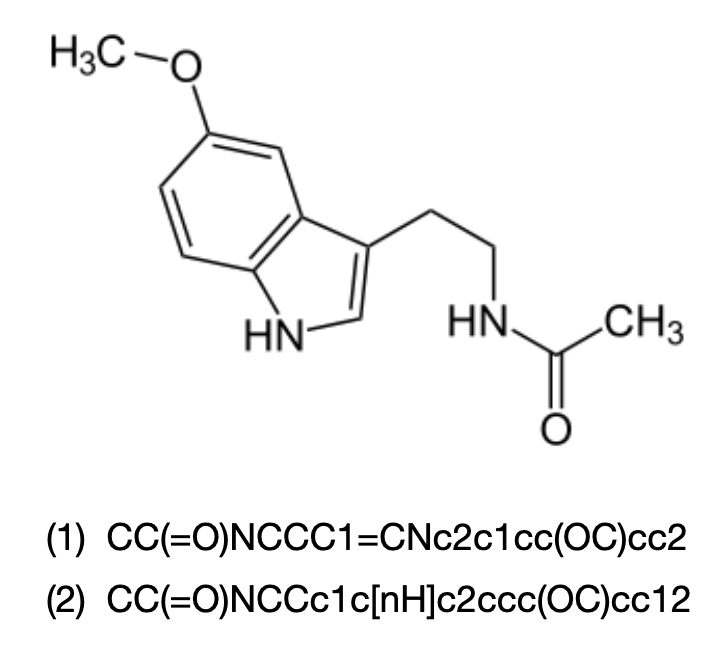
\includegraphics[scale=0.25]{imagenes/smiles_melatonina.png}}  
    \caption{Dos posibles codificaciones de la melatonina en SMILES \cite{smiles_wikipedia}} \label{fig:figura2}
\end{figure}

Aunque no vamos a entrar en detalle de cómo funciona, ya que para ello hay que tener nociones avanzadas de química, diremos que utiliza las siglas de cada elemento de la tabla periódica para representar los átomos. La primera letra del elemento se escribe en mayúscula, a no ser que se trate de un átomo perteneciente a un anillo aromático\footnote{La aromaticidad es una propiedad presente en enlaces dobles de moléculas cíclicas, donde sus electrones pueden circular libremente. Esto mejora la estabilidad del compuesto. \cite{aromaticidad, aromaticidad_wikipedia}}, ya que en ese caso se escribe en minúscula. Si el elemento tiene dos caracteres, el segundo se escribe siempre en minúscula. Además, se pueden representar cargas.

Los enlaces se representan con -, =, \# y :, según el tipo. Bajo algunas circunstancias, se pueden omitir estos símbolos, ya que por su contexto se deducen. También se pueden codificar ramas, situando elementos entre paréntesis, y ciclos, utilizando un número para indicar el inicio y el fin del ciclo en la cadena de texto. \cite{weininger1988smiles}

\begin{figure}[H]
\centering
    \fbox{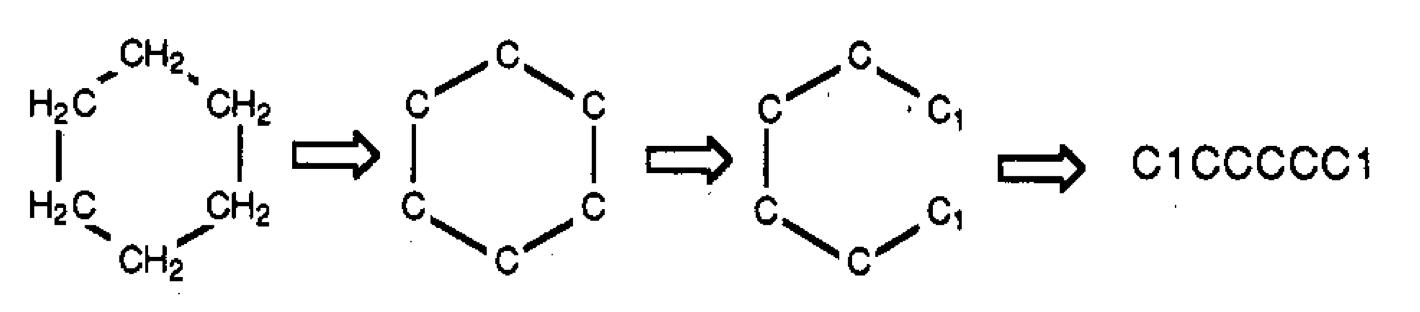
\includegraphics[scale=0.35]{imagenes/smiles_cycle.png}}  
    \caption{Ciclos en SMILES} \label{fig:figura2}
\end{figure}

Otras características como la aromaticidad o estructuras inconectas también pueden ser representadas. Entre las ventajas de esta codificación, destaca su facilidad de comprensión por los humanos. Cualquier químico puede aprender sus reglas de codificación fácilmente y diseñar sus propios compuestos. Un problema que tiene SMILES es que un mismo elemento se puede representar de diferentes formas. Pero sobre todo, el mayor problema es que un porcentaje significativo de las cadenas no se corresponden con moléculas válidas, ya sea porque son sintácticamente inválidas, no se corresponden con un grafo molecular o no cumplen reglas químicas básicas. \cite{weininger1988smiles}

Uno de los principales objetivos de la química computacional es el diseño de nuevas moléculas. Para ello, la utilización de modelos generativos puede ayudar a los investigadores, pero si el espacio de estados de SMILES no es completamente válido se dificulta la tarea. Para ello han surgido otras codificaciones como SELFIES con un espacio 100\% robusto. \cite{Krenn_2020}

Además de estos formatos de notación lineal, es necesario mencionar otros. El lanzamiento en 1982 de MDL Molfile llevó a su aceptación como principal formato para representar datasets químicos. Se han realizado distintas adaptaciones de este para añadir información extra a las moléculas, dando lugar a SDfile, RGfile, Rxnfile, etc. El formato PDB se utiliza principalmente para almacenar información 3D de macromoléculas biológicas, como son las proteínas o los polinucleótidos. CIF también es un formato para almacenar información 3D. En espectroscopia encontramos JCAMP. Finalmente, CML (chemical markup language), una extensión de XML, es una propuesta que intenta aglutinar toda la información disponible. Es compatible con moléculas, reacciones, espectroscopia y otra información. \cite{doi:10.1021/ci600234z}

\begin{figure}[H]
\centering
    \fbox{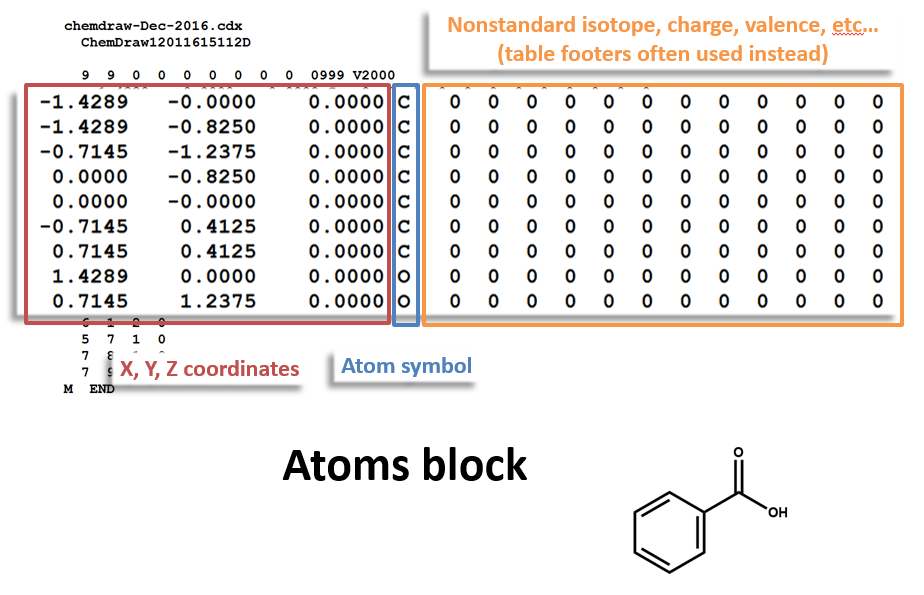
\includegraphics[scale=0.3]{imagenes/molfile.png}}  
    \caption{Contenido de un archivo MOL \cite{molfile_example}} \label{fig:figura2}
\end{figure}


\section*{Fuentes y bases de datos}

El gran número de facetas que presenta la información química necesita sistemas de almacenamiento a la altura. La química fue una de las primeras ramas científicas en utilizar bases de datos para almacenar: la cantidad de datos que se generaba creció rápidamente, y sigue creciendo hoy en día. 

Aunque es muy complicado clasificarlas, vamos a separarlas en tres grandes grupos según el tipo de información que almacenan: \cite{doi:10.1021/ci600234z}
\begin{itemize}
    \item \textbf{Bases de datos de publicaciones:} Pueden ser bibliográficas, guardando solamente los metadatos y la referencia a la publicación, o de texto completo, donde recogen la publicación de forma íntegra. %TODO: Qué son las publicaciones primarias?
    \item \textbf{Bases de datos fácticas:} Al contrario que las anteriores, que almacenan publicaciones de la literatura primaria, estas pueden guardar propiedades físicas de compuestos, información de espectroscopia, información legal, etc.
    \item \textbf{Bases de datos de estructuras y reacciones:} Recogen estructuras químicas, tanto individualmente como formando parte de reacciones. No se almacenan como imágenes, sino en formatos interpretables por la máquina.
    \item \textbf{Bases de datos de biología molecular:} Contienen secuencias de aminoácidos y nucleótidos.
\end{itemize}

Pero, ¿cómo podemos rellenarlas con datos? ¿De dónde podemos extraerlos? Durante décadas se han publicado un gran número de artículos. Podríamos utilizarlos como una fuente muy amplia de información, ya que contienen todo el progreso científico. Específicamente para extraer datos relativos a estructuras, entran en juego utilidades conocidas como OCSR (Optical Chemical Structure Recognition).

Son capaces de transformar una imagen en un formato compatible con la máquina, como podría ser SMILES. En muchos casos incluso es posible introducirles una publicación completa y ellas mismas localizan las imágenes de moléculas. Con el paso del tiempo se han ido perfeccionando, y algunas son capaces de detectar información estereoquímica o de relacionar el compuesto con el texto de la publicación. Más adelante repasaremos algunas de estas utilidades. 

Por último, mencionar una base de datos que merece la pena conocer. Creada por el National Institute of Health (NIH), PubChem es una base de datos abierta que cada mes sirve a millones de usuarios en todo el mundo. Es una base de datos de estructuras y aunque contiene mayoritariamente moléculas pequeñas, también almacena nucleótidos, carbohidratos, lípidos, péptidos y macromoléculas modificadas químicamente. Para cada compuesto almacena su estructura, identificadores, propiedades físicas y químicas, toxicidad, patentes, etc. Los datos que aglutina provienen de diversas fuentes, como son agencias del gobierno estadounidense, editores de revistas científicas o proveedores químicos, aunque hay muchas más. \cite{pubchem}

\section*{Métodos de búsqueda}
Almacenar información en las bases de datos no sirve de nada si no se desarrollan métodos eficientes para extraerla. En aquellas bases de datos donde se almacenan estructuras químicas, una de las principales formas de obtener información es buscar similitudes entre una molécula dada como entrada y otras que se encuentran almacenadas, de forma que compartan una subestructura específica o tengan otras características en común. Para ello, es clave la codificación de los compuestos.

También, si se almacenan metadatos y la base de datos está indexada sobre ellos se podría buscar por su nombre, etiquetas, etc. \cite{doi:10.1021/ci600234z}


\section*{Métodos para análisis de datos}
En química, grandes cantidades de datos son producidas. Una vez que hemos conseguido limpiarlos y ordenarlos, tenemos un conocimiento muy valioso en nuestras manos. La información es muy interesante en sí misma, pero también lo son las relaciones que se esconden en su interior. Para ello, se crean modelos que puedan interiorizarlas.

El análisis de datos no solo se enfrenta a la extracción de la información principal, sino que también intenta generar nueva información secundaria. \cite{doi:10.1021/ci600234z}

Este TFG se desarrolla dentro de este ámbito, ya que, como describiremos más adelante, entrenamos un modelo capaz de detectar que imágenes contienen moléculas organometálicas. Además, creamos un modelo generativo para aumentar el tamaño del dataset en uso.